%%%%%%%%%%%%%%%%%%%%%%%%%%%%%%%%%%%%%%%%%
% a0poster Portrait Poster
% LaTeX Template
% Version 1.0 (22/06/13)
%
% The a0poster class was created by:
% Gerlinde Kettl and Matthias Weiser (tex@kettl.de)
% 
% This template has been downloaded from:
% http://www.LaTeXTemplates.com
%
% License:
% CC BY-NC-SA 3.0 (http://creativecommons.org/licenses/by-nc-sa/3.0/)
%
%%%%%%%%%%%%%%%%%%%%%%%%%%%%%%%%%%%%%%%%%
% Perrinet18gdr
%----------------------------------------------------------------------------------------
%	PACKAGES AND OTHER DOCUMENT CONFIGURATIONS
%----------------------------------------------------------------------------------------
\newcommand{\Author}{Laurent U.~Perrinet$^1$}%
\newcommand{\Address}{$^1$~Institut de Neurosciences de la Timone, CNRS / Aix-Marseille Universit\'e - Marseille, France}%
\newcommand{\Website}{http://invibe.net/LaurentPerrinet}%
\newcommand{\Title}{A low-cost, accessible eye tracking framework}%
\newcommand{\Email}{laurent.perrinet@univ-amu.fr}%

\documentclass[a0,portrait]{a0poster}

\usepackage{multicol} % This is so we can have multiple columns of text side-by-side
\columnsep=100pt % This is the amount of white space between the columns in the poster
\columnseprule=3pt % This is the thickness of the black line between the columns in the poster

\usepackage[svgnames]{xcolor} % Specify colors by their 'svgnames', for a full list of all colors available see here: http://www.latextemplates.com/svgnames-colors

\usepackage{times} % Use the times font
%\usepackage{palatino} % Uncomment to use the Palatino font

\usepackage{graphicx} % Required for including images
\graphicspath{{figures/}} % Location of the graphics files
\usepackage{booktabs} % Top and bottom rules for table
\usepackage[font=small,labelfont=bf]{caption} % Required for specifying captions to tables and figures
\usepackage{amsfonts, amsmath, amsthm, amssymb} % For math fonts, symbols and environments
\usepackage{wrapfig} % Allows wrapping text around tables and figures

\usepackage{natbib}
\begin{document}

%----------------------------------------------------------------------------------------
%	POSTER HEADER 
%----------------------------------------------------------------------------------------

% The header is divided into two boxes:
% The first is 75% wide and houses the title, subtitle, names, university/organization and contact information
% The second is 25% wide and houses a logo for your university/organization or a photo of you
% The widths of these boxes can be easily edited to accommodate your content as you see fit

\begin{minipage}[b]{0.75\linewidth}
%\VeryHuge
\Huge \color{Navy} \textbf{\Title} \color{Black}\\ % Title
%\Huge\textit{Country Update}\\[2.4cm] % Subtitle
\huge \textbf{\Author} \\[0.5cm] % Author(s)
\huge \Address\\[0.4cm] % University/organization
\Large \texttt{\Email} \\
\end{minipage}
%
\begin{minipage}[b]{0.25\linewidth}

\includegraphics[width=13cm]{Logo_int.png}\ 

\includegraphics[width=10.5cm]{Logo_amu.png}\\
\end{minipage}

\vspace{1cm} % A bit of extra whitespace between the header and poster content

%----------------------------------------------------------------------------------------

\begin{multicols}{3} % This is how many columns your poster will be broken into, a portrait poster is generally split into 2 columns

%----------------------------------------------------------------------------------------
%	ABSTRACT
%----------------------------------------------------------------------------------------

\color{Navy} % Navy color for the abstract

\begin{abstract}
Recording eye movements is a technique that attracts an increasing number of scientists, but also in the general public. Indeed, this allows to quantitatively measure a number of useful dimensions of perception and behavior in general. However, most existing trackers rely on expensive or technically complex solutions. Here, we propose a simple framework to record eye movements using any camera, such as a webcam. As a proof of concept, the recorded image is processed in real-time to detect from a simple sub-set of eye movements : left, center, right or blink. The processing is based on two stages. First, we use a pre-trained computer vision algorithm to extract the image of the face. Second, we used a classical deep-learning architecture to learn to classify these sub-images. This network is a 3 layered convolutional neural network, for which we optimized performance as measured by the accuracy with cross-validation on a wide range of the network's hyper-parameters. Over a dataset of more than 1000 images, this network achieves an average accuracy of approximately 97\%. We also provide with an integration with the psychopy library which shows that frames can be processed on a standard laptop at a rate of approximately 25Hz.
\end{abstract}

%----------------------------------------------------------------------------------------
%	INTRODUCTION
%----------------------------------------------------------------------------------------
\color{Black} % SaddleBrown color for the introduction
\section*{Introduction}
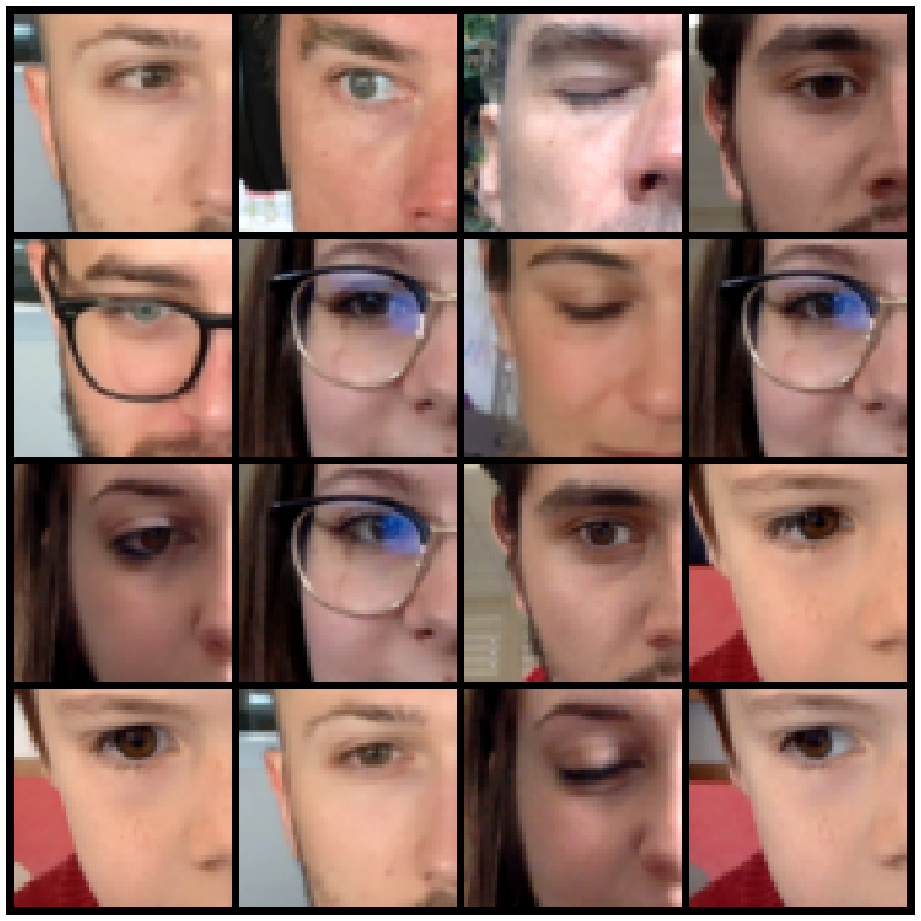
\includegraphics[width=1.\linewidth]{dataset.pdf}
\captionof{figure}{\color{Green} We investigated the performance of a novel, low-cost, low-precision eye tracker.}
%\end{center}%\vspace{1cm}
%----------------------------------------------------------------------------------------
%	Partie ring model
\color{Black} % DarkSlateGray color for the rest of the content
\section*{Recognition model} %ignore the error, they're from my \Inn fonction that works for maths zones
% Notebook partie A
%----------------------------------------------------------------------------------------

Our model was trained on more than 1000 images taken from a webcam. Accuracy was tested on 20 cross-validations.

%\begin{center}\vspace{1cm}
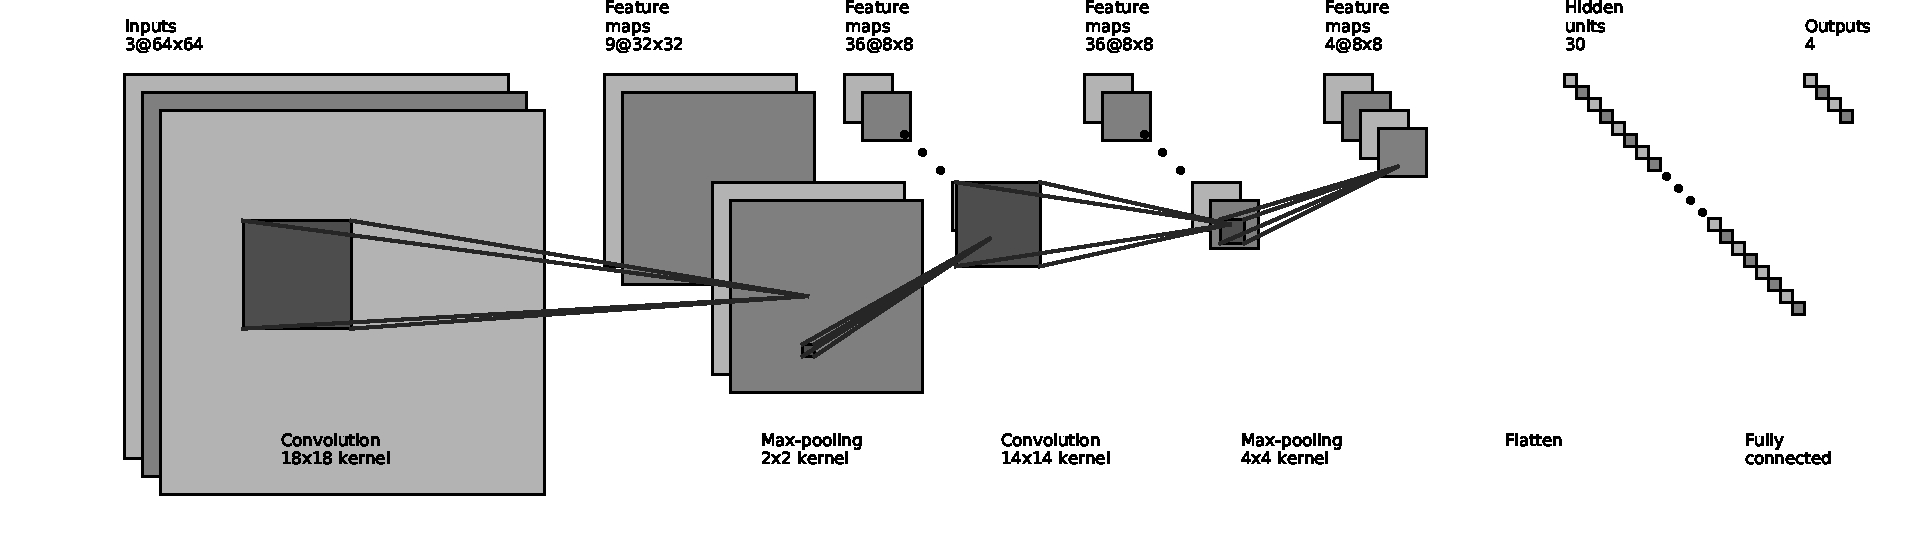
\includegraphics[width=1\linewidth]{CNN.pdf}
\captionof{figure}{\color{Green} The architecture of the original convolutional neural network, as introduced by LeCun et al. (1989), alternates between convolutional layers including rectifying non-linearities and max-pooling layers layers. The feature maps of the final subsampling layer are then fed into two layers of fully connected neurons. The output layer uses softmax activation functions to generate a decision. }

%\end{center}%\vspace{1cm}
%----------------------------------------------------------------------------------------
%	GEOTHERMAL DATA
%----------------------------------------------------------------------------------------
\section*{Psychophysics Data}
\subsection*{2AFC Task}
For our 2-Alternative Forced Choice task (2AFC), subjects were shown two different MotionClouds in quick succession. The first $\theta$ was always 90$^\circ$ (vertical) and the second was randomly chosen to produce a left/right shift. Subjects then had 1000 ms to \textbf{guess the direction of this shift}.
\begin{itemize}
\item For each human trial, $B_\theta$ was randomly chosen out of 7 possibilities and 150 trials were performed.
\item For each model trial, $B_\theta$ was randomly chosen out of 15 possibilities and 600 trials were performed.
\end{itemize}

\begin{center}\vspace{1.2cm}
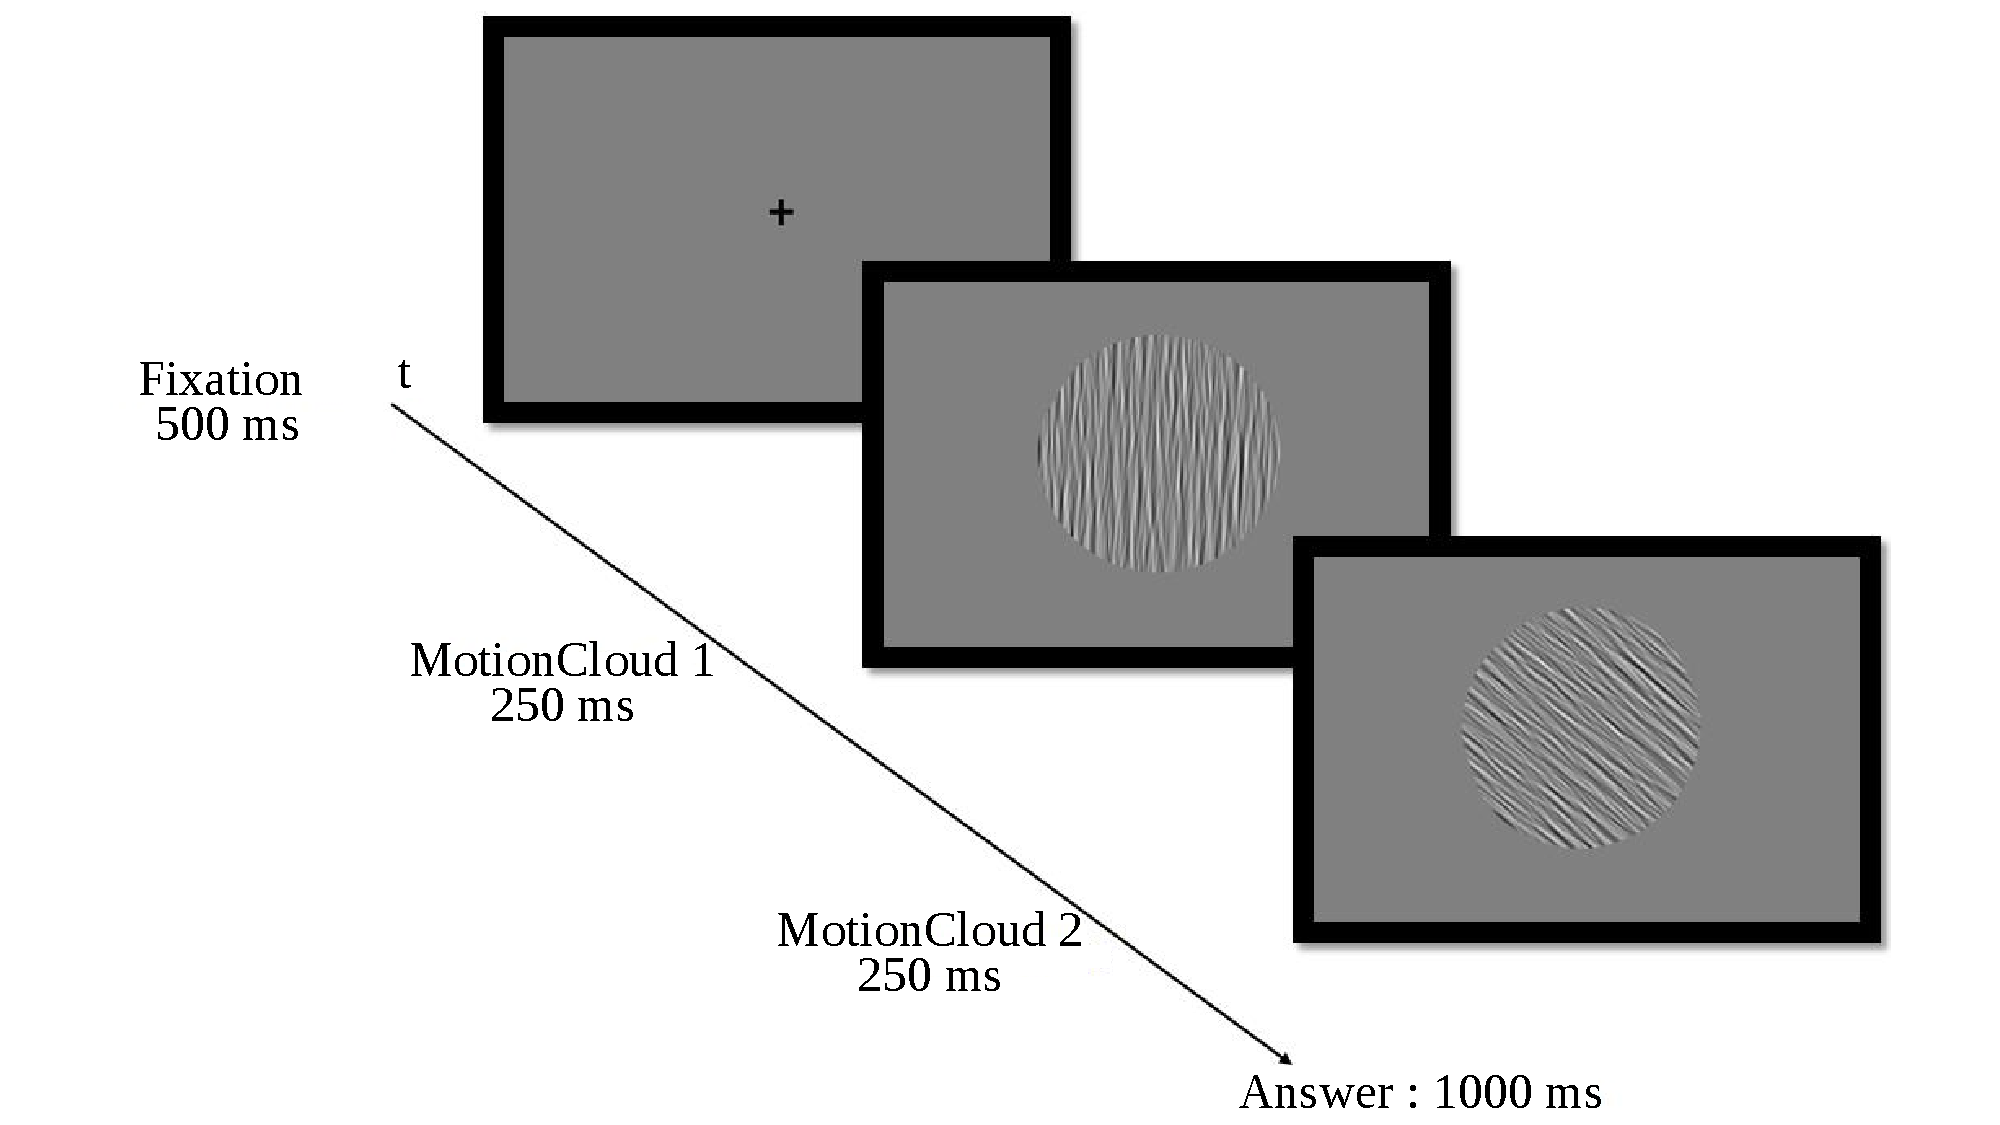
\includegraphics[width=1.\linewidth]{Figure_trial.pdf}
\captionof{figure}{\color{Green} 2AFC task design. After a fixation time, subject were shown two stimulus before having to guess a shift, for a total of 2s per trial. n = 13.}
\end{center}\vspace{1.2cm}

\subsection*{Human vs Model performance}
Accuracy for 2AFC task was best for $B_\theta$ $<$ 28$^\circ$ and underwent a \textbf{rapid, full collapse} for $B_\theta$ $>$ 51$^\circ$, both for humans and model runs. Model accuracy was slightly lower than humans' for all noise level.
\begin{center}\vspace{1cm}
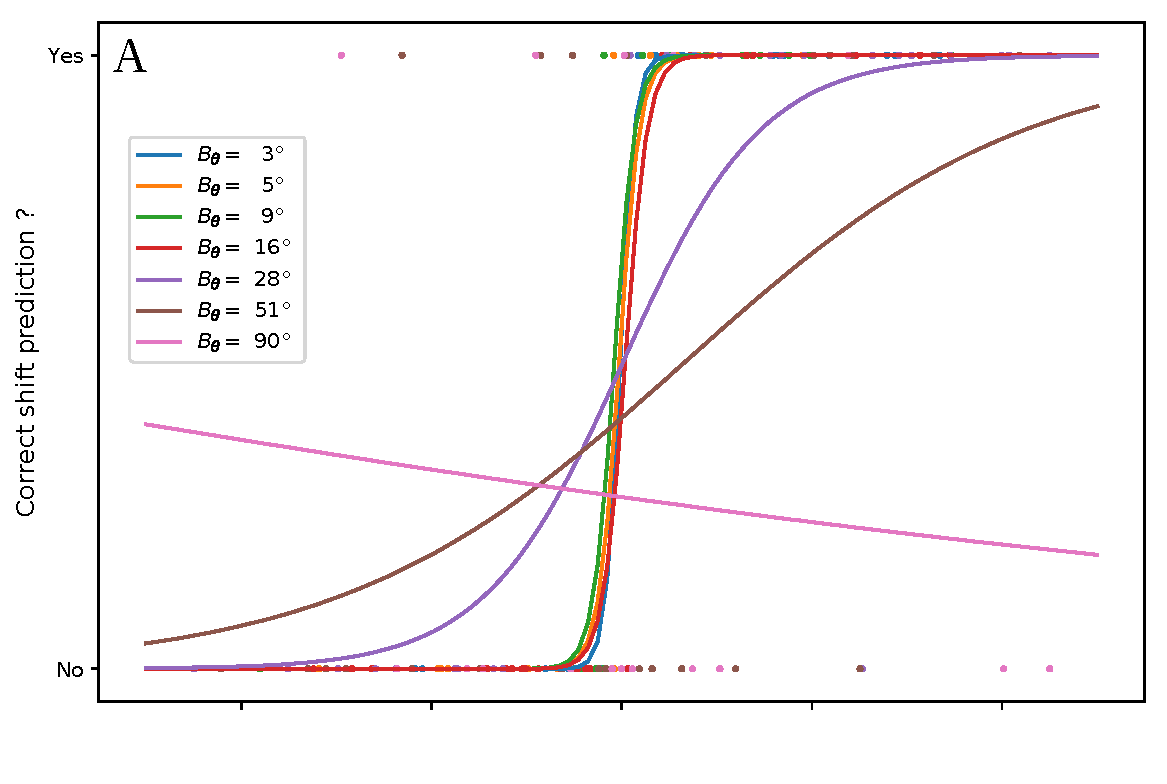
\includegraphics[width=1.\linewidth, page=1]{mergedfigs.pdf}
\includegraphics[width=1.\linewidth, page=2]{mergedfigs.pdf}
\captionof{figure}{\color{Green} Logistic regressions for a randomly picked human subject (A) and Ring Model (B).  }
\end{center}\vspace{1cm}


\subsection*{F1 scores}
We subsequently compared F1 scores, whose distribution furthers our previous interpretation that our model is relevant in approximating human performance in this task.
\\ We then set to investigate the role of lateral connectivity of the primary visual cortex using the model. \textbf{LSTM was deactivated}, leaving the cortical columns without any lateral information, causing a threefold lower F1 score for $B_\theta$ $>$ 40$^\circ$. 
\begin{center}\vspace{1cm}
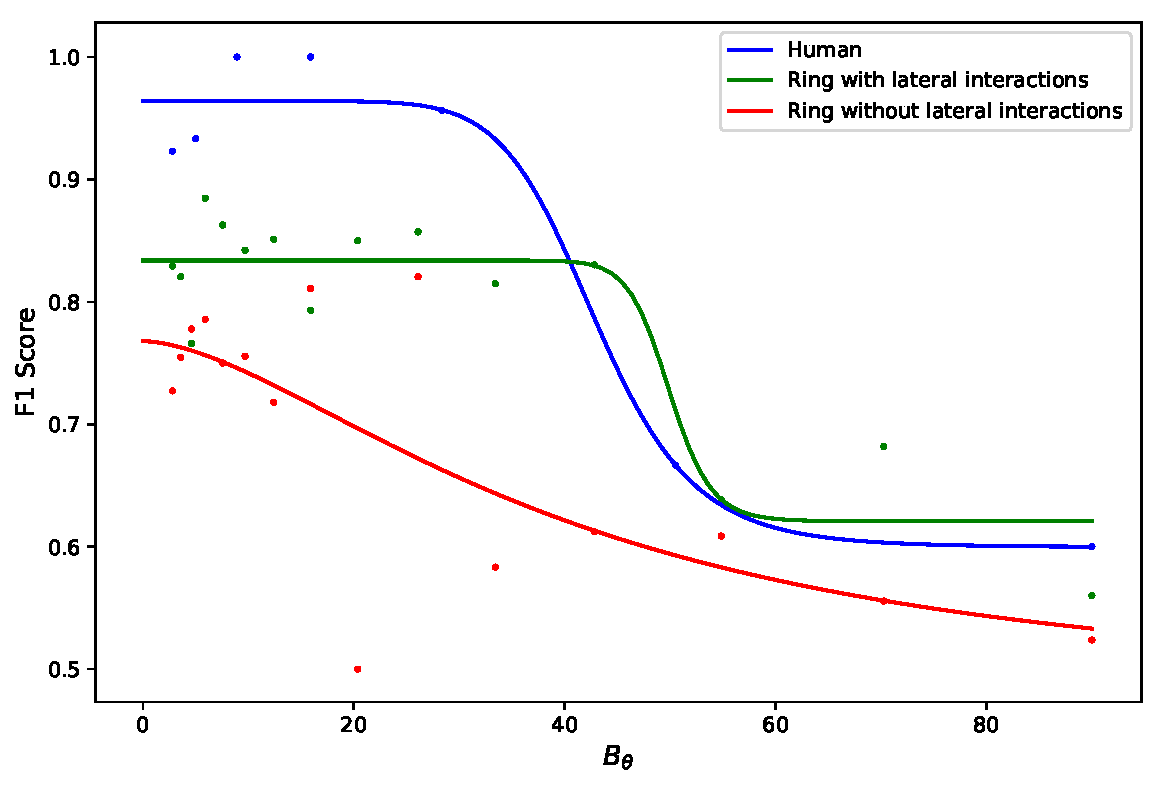
\includegraphics[width=1.\linewidth, page=1]{F1_curve.pdf}
\captionof{figure}{\color{Green} Quadratic logistic regressions for the same randomly picked human subject as Figure 4(A), Ring Model and a Ring Model with an inactive lateral connectivity.}
\end{center}\vspace{1cm}

%\captionof{figure}{\color{Green} Logistic regressions for the ring model. Accuracy is overall lower than humans but collapsed the same way for B$\theta$ $>$ 51$^\circ$. }


%----------------------------------------------------------------------------------------
%	CONCLUSIONS
%----------------------------------------------------------------------------------------

\color{Navy} % SaddleBrown color for the conclusions to make them stand out

\section*{Conclusions}
The visual cortex is canonically described as a group of cortical columns organized in a hierarchical network, whose entry level consists of oriented stimulus in the visual field~\citep{Hubel68}. \\
In this network, the role of lateral connectivity between columns selective to different orientation has often been theorized to be an inhibitor network for neighbouring columns~\citep{BLAKEMORE1970} or a support for contour integration~\citep{Stettler2002}.\\
Here, using a new deep-learning model, we showed that orientation discrimination of the primary visual cortex varies in an 'all or none' fashion past a certain threshold. Suppressing the lateral connectivity of this model resulted in a tremendous F1 loss only for higher $B_\theta$, hence our hypothesis that this lateral connectivity could also increase the robustness of the primary visual cortex to noisy inputs. 
\color{Black} % Set the color back to DarkSlateGray for the rest of the content

%----------------------------------------------------------------------------------------
%	FORTHCOMING RESEARCH
%----------------------------------------------------------------------------------------

%\section*{Forthcoming Research}


%----------------------------------------------------------------------------------------
%	BONUS : Polar plots and QR Code
%----------------------------------------------------------------------------------------
\section*{Additional resources}
\begin{minipage}{0.67\linewidth}
Polar plots of the MotionClouds shown in the Introduction section.
\end{minipage}
\begin{minipage}{0.3\linewidth}
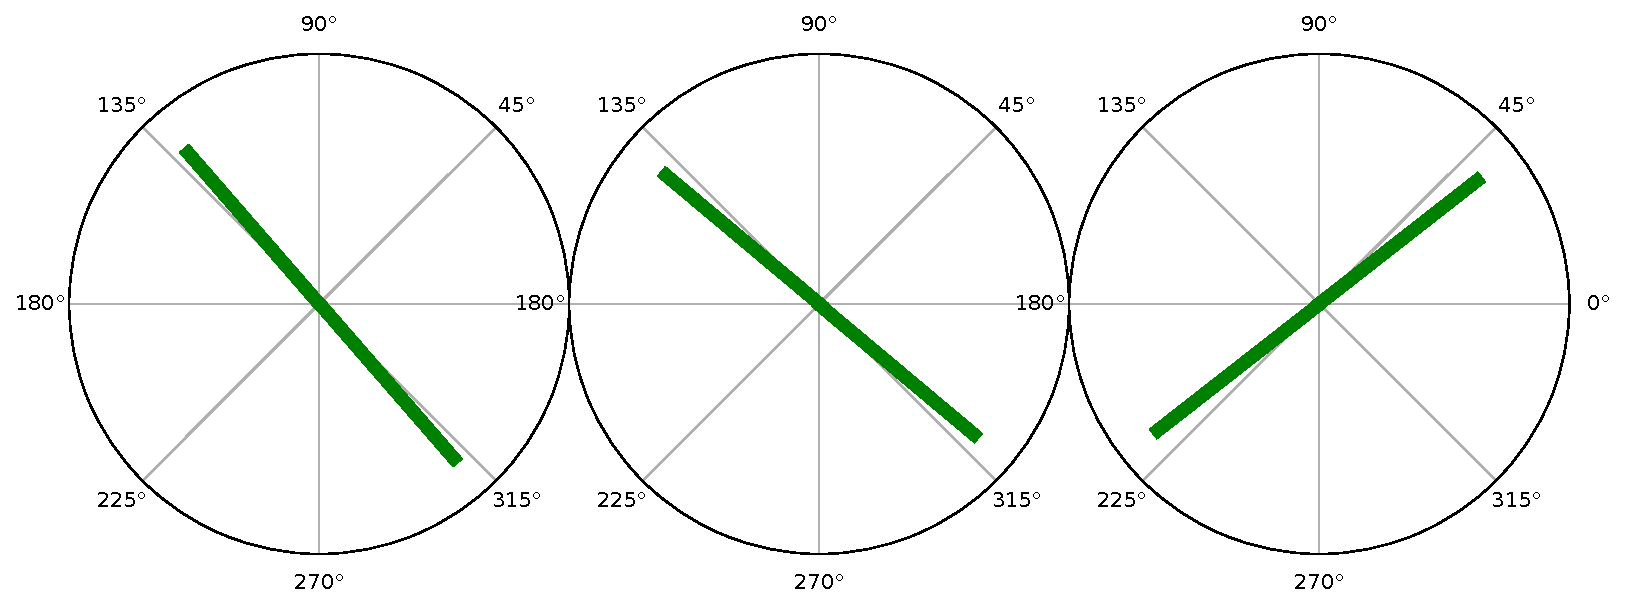
\includegraphics[width=1\linewidth]{Polar_plot_MC1.pdf}
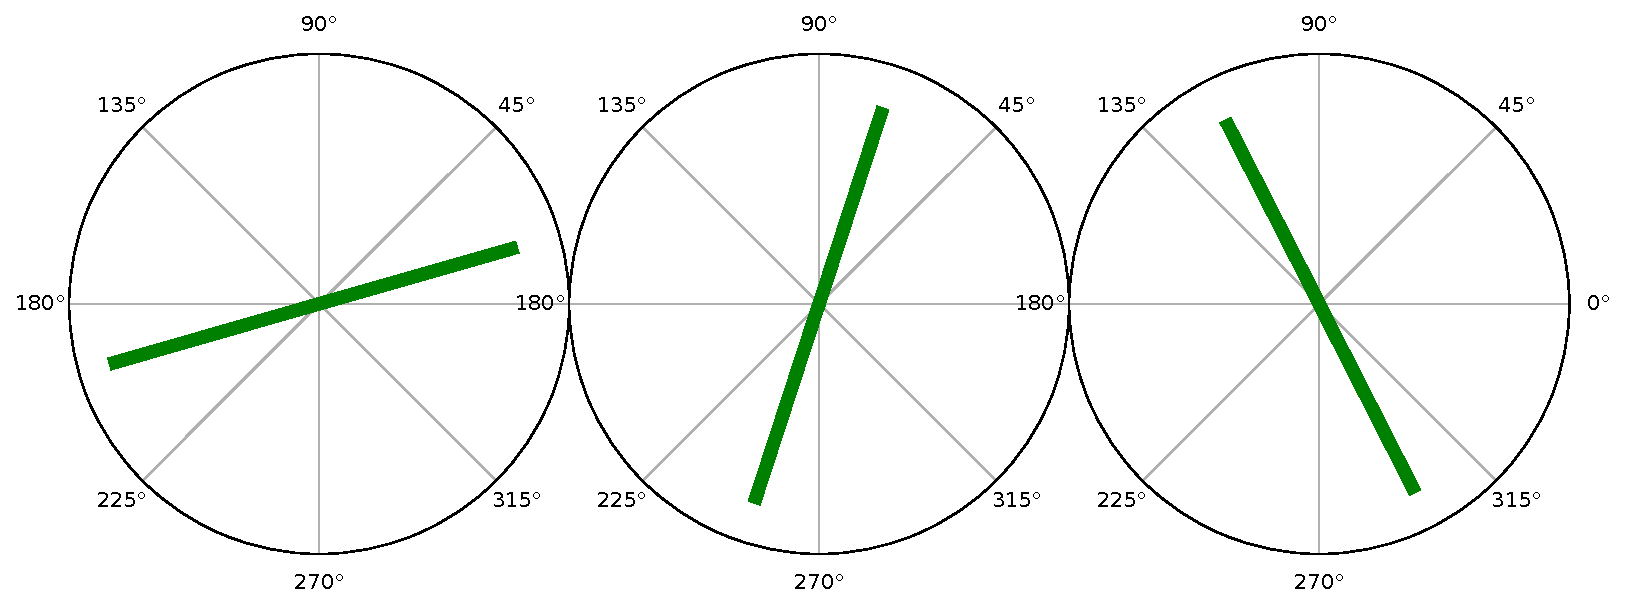
\includegraphics[width=1\linewidth]{Polar_plot_MC2.pdf}
\end{minipage}\hfil

\begin{minipage}{0.3\linewidth}

\includegraphics[width=1.\linewidth]{GitQR.png}
\end{minipage}\hfil
\begin{minipage}{0.67\linewidth}
The model and data are open-source. You can either flash the code or go to www.github.com/hugoladret/InternshipM1 to get them.
\end{minipage}
 %----------------------------------------------------------------------------------------
%	REFERENCES
%----------------------------------------------------------------------------------------
%\nocite{*} % Print all references regardless of whether they were cited in the poster or not
\bibliographystyle{plain} % Plain referencing style
\bibliography{obv1} % Use the example bibliography file sample.bib
%----------------------------------------------------------------------------------------

\end{multicols}
\end{document}